\section{Покази до виконання лапароскопічних резекцій печінки}

Технічні можливості лапароскопічної хірургії постійно зростають а хірургічна техніка вдосконалюється завдяки чому більшість втручаннь, що раніше виконувались лише у відкритому доступі зараз можлива і в лапароскопічному варіанті. Враховуючи сучасні досягнення покази до \acrshort{llr} практично не відрізняються від показів до \acrshort{olr} - лапароскопічний досуп не обмежує хірургічні можливості, проте додає певні, властиві саме йому, особливості. 

Серед показів до резекції печінки розрізняють злоякісну та доброякісну патологію. Серед онкопатології, на долю якої приходиться 60-80\% резекцій  найбільш частими показами до хірургічного лікування є первинні пухлини печінки та жовчних шляхів, а саме гепатоцелюлярна карцинома (\acrshort{hcc}), внутрішньопечінкова (або масформуюча) холангіокарцинома (\acrshort{ihcc}), перихіларна холангіокарцинома (\acrshort{phcc}), рак жовчного міхура (\acrshort{gbc}) та метастази колоректального раку в печінку \acrshort{crlm}. 
В цьому розділі ми зосередимось на тих видах хірургічної патології печінки, при яких застосування мініінвазивного підходу дає можливість отримати позитивні результати. 

\subsection{Гепатоцеллюларна карцинома}.
Гепатоцеллюлярна карцинома (\acrshort{hcc}) є п'ятою за частотою серед причин летальності від онкологічних захворюваннь. Причиною цього є  виявлення пізніх стадій захворювання через його асимптоматичний перебіг. Поширені форми \acrshort{hcc} характеризуються судинною інвазією, яка значно утруднює їх хірургічне лікування, а також наявністю у більшості хворих супутнього хронічного захворювання печінки та цирозу які суттєво погіршують печінкову функцію. Окрім того \acrshort{hcc} є хіміорезистентною пухлиною, що робить системну хіміотерапію не ефективною.

Сучасний підхід до лікування \acrshort{hcc} базується на виборі методу лікування в залежності від стадії пухлини. Найбільш часто вживаною системою стаціювання \acrshort{hcc} є барселонська (\acrfull{bclc}, \acrshort{bclc}) \cite{Llovet2003}. Згідно \acrshort{bclc} хірургічне лікування показано на ранній та дуже ранній стадіях \acrshort{hcc}, коли пухлина представлена солітарними резектабельними вузлами, а можливми опціями лікування є етанолова або радіочастотна абляція, відкрита або лапароскопічна резекція та трансплантація печінки. 

При дуже ранній стадії \acrshort{hcc} за \acrshort{bclc} з розміром вогнища до 2 см найбільш ефективні етанолова та радіочастотна абляція  \cite{Cucchetti2013}. Пацієнтам з \acrshort{hcc} в межах міланських критеріїв та декомпенсованим цирозом печінки оптимальним методом лікування є трансплантація печінки \cite{Colombo2016}. Для всіх інших пацієнтів з резектабельними формами \acrshort{hcc} методом першого вибору є резекція печінки \cite{Heimbach2018, Kudo2011}. 

\subsubsection{Анатомічні та неанатомічні резекціії з приводу \acrshort{hcc}}

\acrshort{hcc} --- агресивна високоінвазивна пухлина, яка має тенденцію до ураження малих та великих внутрішньопечінкових судин, периваскулярних компартментів та жовчних шляхів. Портальні тромби спричинені судинною інвазією можуть викликати кавернозну трансформацію та перивенозну колатеральну сітку. Мікросудинна інвазія це типова особливість \acrshort{hcc}, характерна переважно менш діфференційованим пухлинам, яка підтверджує агрессивну біологію пухлини. Незалежними предикторами мікроваскулярної інвазії є розмір пухлини більший 5 см., та менший ступінь дифференціації \cite{Zimmermann2017}. Інвазія в дрібні внутрішньопечінкові гілки ворітної вени може приводити до локального ретропортального кровотоку та периферійного внутрішньопечінкового розповсюдження у вигляді числених метастатичних вузлів по ходу судин в межах портального судинного басейну локальної анатомічної ділянки (Рис. \ref{fig:HCC_vascular_invasion}). 


\begin{figure}[h]
\caption{Механізм виникнення пухлинного портального тромбозу при ГЦК}
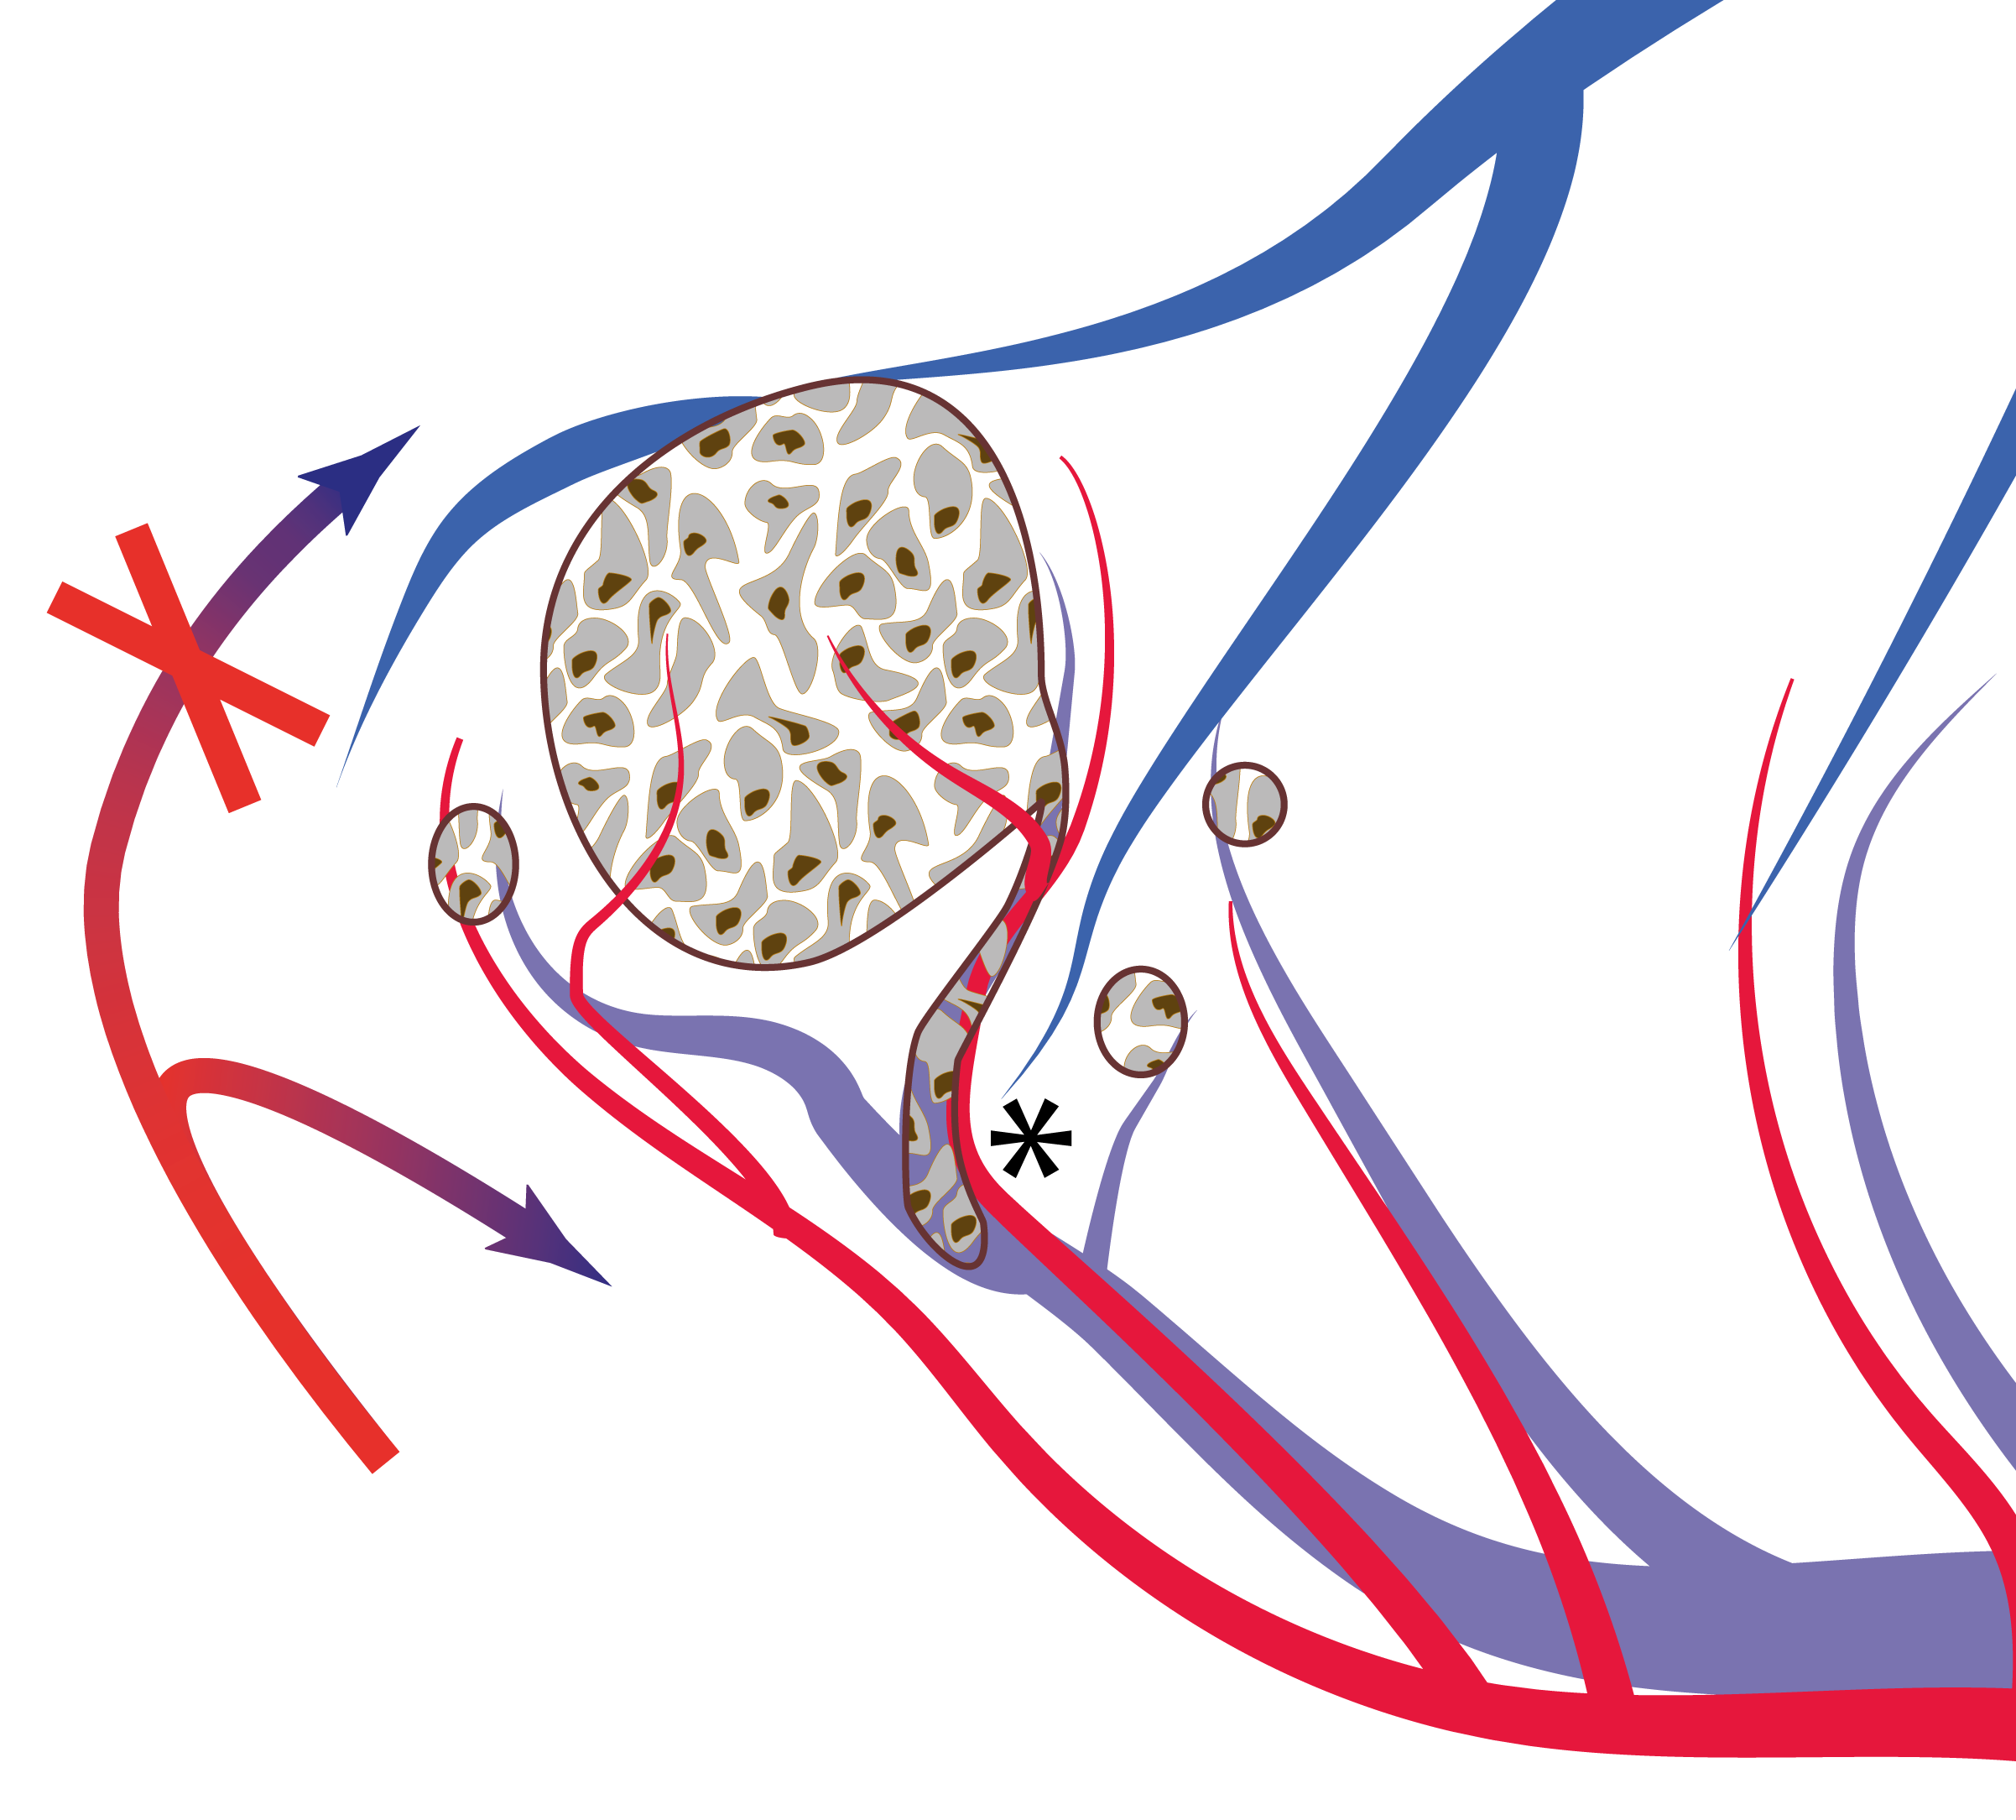
\includegraphics[width=0.9\textwidth]{Illustrations/Chapter_01/HCC_vascular_invasion.png}
\label{fig:HCC_vascular_invasion}

\medskip
\small
Під час свого росту пухлина інвазує дрібні гілки печінкових вен та створює локальну венозну гіпертерзію. Це призводить до локального реверсу кровотоку (помічено стрілками) в портальних гілках та росту пухлинного тромбу (помічено зірочкою) проти напрямку портального кровотоку.

\end{figure}




Враховуючи схильність \acrshort{hcc} до локального метастазування в межах анатомічних ділянок методом вибору хірургічного лікування є анатомічна резекція печінки (\acrshort{alr}). На відміну від неанатомічної резекції печінки (\acrshort{non-alr}) \acrshort{alr} включає в себе ідентифікацію судинного бассейну анатомічної ділянки, що містить пухлину та видалення всієї її паренхіми. Онкологічні переваги \acrshort{alr} підтверждують більшість дослідженнь, так Makuuchi M. та співавтори \cite{Shindoh2016} в дослідженні 209 пацієнтів з цирозом класу А за Чайлдом та \acrshort{hcc} розміром $\leq$ 5 см, що були резектабельні як за допомогою \acrshort{alr} так і \acrshort{non-alr} показали перевагу \acrshort{alr} завдяки меншому ризику локальних рецидивів та більшій тривалості життя. Автори метааналізу \cite{Moris2018} 43 досліджень стверджують, що у 6839 пацієнтів яким була виконана \acrshort{alr} в порівнянні з 5590 пацієнтами з \acrshort{non-alr} були кращі загальна та безрецидивна виживаність та морбідність та рання післяопераційна летальність.

До переваг \acrshort{alr} відносять кращий онкологічний ефект, а до недоліків - вищий порівняно з \acrshort{non-alr} ризик післяопераційного порушення печінкової функції, пов'язаний з більшим об'ємом резекції, що особливо важливо для пацієнтів із цирозом печінки. Враховуючи це необхідний ретельний відбір пацієнтів для резекції печінки з приводу \acrshort{hcc}, що базується на оцінці рівню печінкової недостатності, ступеню портальної гіпертензії та загального статусу пацієнта. Американські клінічні настанови National Comprehensive Cancer Network (\acrshort{NCCN}) в якості кандидатів для резекції печінки пропонують пацієнтів з компенсованою печінковою функцією, солітарним вогнищем без макросудинної інвазії та майбутнім печінковим залишком (\acrshort{flr}) $\geq$ 20\% для здорової паренхіми та $\geq$ 30-40\% з адекватним кровопостачанням та жовчевідтоком. В клінічних настановах Європейської ассоціації вивчення хвороб печінки по лікуванню \acrshort{hcc} \cite{Galle2018a} для пацієнтів з цирозом печінки запропоновано спрощений алгорим визначення ризику \acrshort{alr}, що базується на об'ємі резекції, супеню портальної гіпертензії та печінкової недостатності. 


\begin{figure}[h]
\caption{Анатомічна резекція Sg 5 печінки з приводу \acrshort{hcc} у виконанні авторів}

\includegraphics[width=0.9\textwidth]{Illustrations/Chapter_01/HCC-Sg5.png}
\label{fig:HCC-Sg5}

\medskip
\small
а) Передопераційні \acrshort{mri} та \acrshort{ct}. Пухлина локалізована в Sg 5 печінки б) Діафрагмальна поверхня Sg 5 печінки з пухлиною  в) Транссекція паренхіми г) Резекційна поверхня ґ, д) Макропрепарат (зірочкою помічено приток від Sg 5 до правої печінкової вени, стрілками - культі сегментарних глісонів)

\end{figure}



\subsubsection{Вибір між лапароскопічною та відкритою резекцією печінки при \acrshort{hcc}} 
Окрім віддалених результатів на ефективність лікування впливає післяопераційна морбідність. Першим з двох основних факторів, які впливають на післяопераційні результати під час резекції печінки з приводу \acrshort{hcc} є крововтрата. Вищий об'єм крововтрати та замісної трансфузії препаратів крові асоційований з вищою з частотою післяопераційних ускладненнь та меншою віддаленою виживаністю \cite{DeBoer2007, Romano2012}. Крововтрата викликає імунодепрессію що сприяє розвитку хірургічних інфекцій, сепсису і збільшення ризику рецидиву в подальшому. Другим фактором є післяопераційна асцитопродукція у пацієнтів з цирозом печінки, яка є грізним ускладненням, що може призводити до великих втрат білка та рідини (до 5 літрів на добу), нагноєння післяопераційної рани та погіршання печінкової функції \cite{Ishii2014}. Окрім збільшення резистивності портального русла через його зменшення внаслідок резекції печінки та набряку печінкового залишку, механізм виникнення асцитопродукції пов'язують з декомпенсацією портальної гіпертензії внаслідок переривання портосистемної колатералізації під час лапаротомії \cite{Kanazawa2013}. 

Згідно існуючих даних, лапароскопічний підхід ефективно знижує ризики обох цих ускладненнь. За рахунок більш прецизійної техніки та позитивного тиску карбоксиперитонеуму \acrshort{llr} асоційовані з меншою інтраопераційною крововтратою, а збереження цілісності колатералей передньої черевної стінки дозволяє знизити частоту та інтенсивність післяопераційної асцитопродукції \cite{Truant2011}. Також \acrshort{llr} зменшують і загальну післяопераційну морбідніть у пацієнтів з \acrshort{hcc} на фоні цирозу при вираженій портальній гіпертензії та тромбоцитопенії < 100,000/мл про що свідчать результати міжнародного мультицентрового порівняльного псевдорандомізованого дослідження результатів лікування 1974 пацієнтів \cite{Ruzzenente2020}.

\emph{Враховуючи наведене вище оптимальними показами до \acrshort{llr} при \acrshort{hcc} є резектабельні форми пухлини всіх локалізацій без ураження магістральних судин або жовчних протоків на фоні здорової паренхіми або компенсованого цирозу печінки при відсутності показів до трансплантації печінки.}

\subsection{Рак біліарного тракту}

Рак біліарного тракту (\acrshort{btc}) - гетерогенна група захворюваннь до якої відносять внутрішньопечінкову (або масформуючу) холангіокарциному (\acrshort{ihcc}), перихіларну холангіокарциному (\acrshort{phcc}), рак жовчного міхура (\acrshort{gbc}) покази до лікування яких за допомогою \acrshort{llr} будуть розглянуті нижче, та рак дистального відділу холедоха і ампулярний рак, які не відносяться до теми цієї книги. 

\subsubsection{Внутрішньопечінкова масформуюча холангіокарцинома}

\acrshort{ihcc} є другою за частотою формою первинного рака печінки з високим потенціалом диссемінації та рецидивів, що походить із клітин проксимальних гілок жовчних протоків, на долю якої припадає до 40\% первинних пухлин печінки. Резекція печінки (Рис. \ref{fig:IHCC}) є єдиним потенційно радикальним методом та застосовується в якості першого етапу лікування \acrshort{ihcc}. Медіана виживаності пацієнтів після радикальної резекції складає 27 - 36 міс \cite{Buettner2017}. Не дивлячись на те, що вплив лімфаденектомії на виживаність при \acrshort{ihcc} остаточно не доказано рекомнедується її рутинне виконання з метою стадіювання процесу та вибору подальшого лікування. При досягненні R0 резекцийного краю необхідна системна адьювантна хіміотерапія, яка може бути доповнена хеморадіаційними методами в разі R1 резекції або позитивних лімфовузлів. При досягненні R2 резекцийного краю із макроскопічними залишками пухлини подальше лікування пацієнта необхідно проводити згідно рекомендацій до лікування нерезектабельних форм \acrshort{ihcc}. 


\begin{figure}[h]
\caption{Лівобічна латеральна секцієеткомія з приводу \acrshort{ihcc} у виконанні авторів}


\includegraphics[width=0.9\textwidth]{Illustrations/Chapter_01/IHCC.png}
\label{fig:IHCC}

\medskip
\small
а) Передопераційне \acrshort{ct}. Пухлина локалізована в Sg 2,3 печінки б) Ліва латеральна секція печінки з пухлиною  в) Транссекція паренхіми (зірочкою відмічені культі сегментарних глісонів, білою стрілкою відмічена культя лівої печінкової вени)  г) Макропрепарат 

\end{figure}

Резекція печінки при \acrshort{ihcc} є комплексною процедурою, технічна складність якої посилюється лімфаденектомією та можливою резекцією позапечінкових жовчних шляхів. Не дивлячись на те, що Саузґемптонські рекомендації не визначають однозначно місце \acrshort{llr} в лікуванні \acrshort{ihcc} через обмежену кількість накопиченого досвіду внаслідок низької частоти резектабельних форм, існує кілька порівняльних дослідженнь, що свідчать на користь лапароскопічного доступу. Так, група південнокорейських авторів на основі порівняння результатів 14 \acrshort{llr} з результатами 23 \acrshort{olr} у пацієнтів з \acrshort{ihcc} зазначає, що при порівняних онкологічних результатах пацієнти, що перенесли \acrshort{llr} мали меншу крововтрату та кращі ранні післяопераційні показники \cite{Lee2016a}. Характерною особливістю дослідження є те, що в нього включені лише невеликі пухлини, розміром $\leq$ 5 см. Ці данні також підтверджує двоцентрове псевдорандомізоване дослідження групи італійських та англійських вчених, в якому на основі вивчення результатів 208 \acrshort{llr} та \acrshort{olr} автори визначають \acrshort{llr} у відібраних пацієнтів  з \acrshort{ihcc}, як доступну та онкологічно ефективну процедуру, асоційовану з меншим ризиком післяопераційних ускладненнь \cite{Ratti2020}.


\subsubsection{Перихіларна холангіокарцинома}

На відміну від інших видів \acrshort{btc}, \acrshort{phcc}, це захворювання при якому показана можливість 10-річної виживаності після хірургічного лікування на рівні 14\% при адекватному відборі пацієнтв \cite{Juntermanns2019}. Через свої біологічні особливості \acrshort{phcc} має схильність до підслизового інфільтративного росту \cite{Sakamoto1998}, що обумовлює поширення пухлини за межі макроскопічно ураження, а також до інвазії магістральних судин ще до клінічної маніфестації у вигляді механічної жовтяниці \cite{Shimada2003}. Пухлина частіше розповсюджується лімфогенним та периневральним, ніж гематогенним шляхом \cite{Zimmermann2017}. Ці морфологічні особливості визначають агресивну хірургічну тактику та об'єм  втручання при \acrshort{phcc}, яке включає резекцію печінки відповідно рівню ураження із тотальною каудальною лобектомією, резекцію позапечінкових жовчних шляхів та розширену лімфаденектомію. За необхідості втручання може бути доповнене резекцією ворітної вени та печінкової артерії при їх пухлинній інвазії а також панкреатодуоденальною резекцією при інвазії дистального края холедоха \cite{Mizuno2019}. 

Через обширність та складність втручання в літературі доступні обмежені данні про мініінвазивне оперативне лікування \acrshort{phcc}. За данними огляду літератури та метааналізу групою авторів з нідерландів у 15 джерелах загалом виявлено 142 випадки виконання радикального мініінвазивного втручання з приводу \acrshort{phcc}, з яких 82 були \acrshort{llr} і 59 робот-асистованими резекціями \cite{Mizuno2019}. Дослідження виявило, що мініінвазивний підхід дає можливість отримати післяопераційну морбідність на рівні 24\% та летальність на рівні 3\%, що порівняно з результатами відкритих резекцій, та досягнути R0 резекції у 80\%. Не зважаючи на отримані оптимістичні результати, автори досить стримані у висновках, що обумовлено недостатньою кількістю накопиченого в світі досвіду та можливістю систематичної похибки через оцінку невеликих ретельно відібраних серій випадків. 

\subsubsection{Рак жовчного міхура}

\acrshort{gbc} є найбільш агресивною формою \acrshort{btc} з медіаною виживаності без лікування 6-10 місяців \cite{Lindner2018}, що пов'язано із асимптоматичним перебігом та пізнім виявленням. Радикальне хірургічна резекція може покращити результати виживаності із досягненням медіани 32 місяців. Сучасна тактика вибору об'єму хірургічного лікування \acrshort{gbc}, зазначена в рекомендаціях \acrshort{NCCN} з лікування гепатобіліарного раку, базується на стадії захворювання та обставинах його виявлення. При аксідентальному виявленні резектабельної ранньої форми \acrshort{gbc} під час холецистектомії остання доповнюється резекцією ложа жовчного міхура печінки або резекцією оточуючих сегментів (Рис. \ref{fig:GBC}). При виявленні пухлини під час планової проводки гістологічного препарату на стадії T1a (без інвазії підслизового шару) рекомендовано подальше спостереження, а на стадії T1b та вище, то в залежності від об'єму інвазії в паренхіму рекомендовано виконання другим етапом резекції Sg 4a-5 печінки або правобічної трисекцієектомії з лімфаденектомією. Резекція позапечінкових жовчних шляхів виконується в залежності від наявності ураження дистального краю міхурової протоки. Виконання резекції позапечінкових жовчних шляхів з метою розширення об'єму лімфаденектомії не є виправданим.  При доопераційному виявленні \acrshort{gbc} план втручання обирається в залежності від об'єму ураження.

В рекомендаціях по лікуванню \acrshort{btc} японської спілки гепатобіліарних хірургів 2015 року зазначається, що \acrshort{gbc} є протипоказом до лапароскопічної холецистектомії у зв'язку із високим ризиком диссемінації та портових метастазів \cite{Miyazaki2015}. Проте в більш пізньому міжнародному експертному консенсусі з лапароскопічної хірургії \acrshort{gbc} 2019 року наголошується, що лапароскопічний доступ не асоційований із погіршенням виживаності при ранніх стадіях \acrshort{gbc} (Т1,Т2) не ассоційованого із гострим холециститом, якщо виконується радикальна резекція, а доведеною причиною диссемінації є пошкодження цілісності стінки жовчного міхура та видалення макропрепарату без використання контейнера. У висновках консенсуса зазначається, що незважаючи на те, що \acrshort{llr} при \acrshort{gbc} є втручанням на ранніх стадіях вивчення, вона не погіршує прогноз, а у ретельно відібраних пацієнтів може покращувати результат операції. 

\begin{figure}[h]
\caption{Резекція Sg 4a,5 з приводу малігнізованого поліпу дна жовчного міхура із інвазією в паренхіму Sg 4 печінки у виконанні авторів}
\centering

\includegraphics[width=0.9\textwidth]{Illustrations/Chapter_01/GBC.png}
\label{fig:GBC}

\medskip
\small
а) Передопераційне \acrshort{ct} та \acrshort{mri}. Пухлина дна міхура (відмічено зірочкою) інвазує в Sg 4a. б) Пухлина контурується в проекції дна жовчного міхура (відмічено зірочкою)  в) Лінія транссекції паренхіми (позначена стрілками)  г) Площина резекції після видалення макропрепарату 

\end{figure}



\emph{Таким чином, на теперішній момент \acrshort{llr} при всіх видах \acrshort{btc} є новою перспективною методикою на етапі вивчення, тому виконання цих операцій обмежено спеціалізованими центрами гепатобіліарної хірургії з великим досвідом мініінвазивних втручаннь.}

\subsection{Метастатичні ураження печінки}

Другим за частотою після первинних пухлин печінки показом до \acrshort{llr}, є метастатичні ураження печінки. До них відносять метастази колоректального раку в печінку (\acrshort{crlm}) та метастази не колоректального походження (нейроендокринні, молочної залози та ін.)


\subsubsection{Метастази колоректального раку в печінку}

Виживаність пацієнтів з \acrshort{crlm} за останні дві декади прогресивно покращилась в результаті запровадження мультидисциплінарного підходу до лікування. Золотим стандартом лікування \acrshort{crlm} є резекція печінки, проте не дивлячись на досягнення сучасної резекційної хірургії лише 25\% пацієнтів мають резектабельні форми ураження на етапі первинної діагностики. Застосування сучасних режимів неоадьювантної хіміотерапії з урахуванням генетичного статусу дозволяє конвертувати до 40-50\% первинно нерезектабельних пацієнтів та виконати радикальну резекцію печінки та позапечінкових ураженнь із задовільною виживаністю \cite{Adam2019a}. 

При оцінці резектабельності принциповим є не кількість та локалізація ураженнь а об'єм та умови функціонування майбутнього печінкового залишку \cite{Allard2017}. Окрім того, враховуючи системну природу захворювання сама по собі пухлинна судинна або позаорганна інвазія не є протипоказом до хірургічного лікування, так як вона не є маркером генералізації процесу та не впливає на прогноз. У більшості випадків судини можуть бути відокремлені від пухлини або доступна судинна резекція \cite{Torzilli2017}. Враховуючи наведене вище агресивний хірургічний підхід при множинних білобарних ураженнях із ураженням магістральних судин печінки або позапечінковою інвазією є обгрунтованим при можливості досягнення R0 резекції (Рис. \ref{fig:CRLM1}).

\begin{figure}[!ht]
\caption{Резекція Sg 7 із резекцією правого купола діафрагми та енуклеорезекцією Sg 8 у пацієнта з рецидивуючим \acrshort{crlm}}

\includegraphics[width=0.9\textwidth]{Illustrations/Chapter_01/CRLM1.png}
\label{fig:CRLM1}

\medskip
\small
а) Передопераційне \acrshort{ct} та \acrshort{mri}. Рецидивні \acrshort{crlm} після неповної черезшкірної абляції (позначені зірочками). В анамнезі відкрита резекція Sg2-3 печінки. б) Місце інвазії метастаза в діафрагму (відмічено стрілкою)  в) Ушивання дефекту діафрмагми після резекції (відмічено стрілками)  г) Лінія транссекції вздовж меж Sg7. ґ) Площина резекції після видалення макропрепарату д) Енуклеорезекція Sg8. е,ж) Макропрепарат. є) КТ через 3 місяці після операції.

\end{figure}


\acrshort{llr} показали себе як ефективний метод лікування \acrshort{crlm}, що підтрержджують результати багатьох порівняльних мультицентрових та рандомізованих досліджень. Так італійське псевдорандомізоване порівняльне дослідження великої когорти пацієнтів (187 \acrshort{llr} проти 698 \acrshort{olr})  показало переваги мініінвазивних втручаннь над відкритими завдяки покращенню ранніх післяопераційних та віддалених результатів (збільшення медіани безрецидивної та загальної виживаності, менший відсоток рецидивів) \cite{Ratti2018a}. Покращена візуалізація та карбоксиперитонеум дозволяють зменшити крововтрату, що позитивно впливає на загальну кількість післяопераційних ускладненнь. Також за данними двох рандомізованих досліджень \acrshort{llr} знижує загальну запальну відповідь, що також зменшує частоту ускладненнь \cite{Kasai2018, Fretland2015}. Також на користь переваг \acrshort{llr} в показниках летальності, морбідності, чистоті резекційного краю та терміну перебування в стаціонарі свідчать результати великого рандомізованого дослідження OSLO-COMET \cite{Fretland2018a}. Окрім того \acrshort{llr} показали свою ефективність при симультантних резекціях первинного вогнища та \acrshort{crlm} \cite{Moris2019}.

Вважається, що на віддалені результати після резекції впливають скоріше біологічні властивості пухлини, ніж ширина резекційного краю. Більшість сучасних дослідників визначає R0 резекцію, як можливість досягнення резекційного краю $\geq$ 1 мм. В окремих дослідженнях показано, що R1 резекції хоча і асоційовані порівняно із R0 із вищою частотою рецидивів, проте лише незначно знижують загальну виживаність \cite{DeHaas2008}. Враховуючи це, оптимальним об'ємом хірургічного лікування \acrshort{crlm} є економні паренхімо-зберігаючі резекції \cite{Matsumura2016, Moris2017}. Використання лапароскопічного підходу для паренхімо-зберігаючих резекцій \acrshort{crlm} дає можливість досягнути до 44\% 5-річної виживаності \cite{Aghayan2018}. Також показана можливість отримання позитивних результатів від лапароскопічного доступу при виконанні двоетапних резекцій та \acrshort{alpps} при білобарному ураженні \acrshort{crlm} \cite{Okumura2019, Melandro2019}.

Загальний ризик рецидиву \acrshort{crlm} після резекції печінки сягає до 60\%. Моноцентрове дослідження результатів лікування 1036 пацієнтів показало, що хірургічне лікування рецидивів \acrshort{crlm} ефективне, так як  довгострокова виживаність пацієнтів після повторних резекцій порівняна з вижвиваністю після первинної резекції печінкових метастазів \cite{Wicherts2013}. Збереження максимальної кількості здорової паренїіми під час \acrshort{llr} не тільки зменшує кількість ускдадненнь, а й збільшує шанси на повторну резекцію у разі рецидиву. Також автори дослідження вказують на те, що повторні \acrshort{llr} асоційовані із зменшенням крововтрати та часу операції порівняно з повторними \acrshort{olr} що також підтвержджує і наш досвід (Рис. \ref{fig:CRLM2}).

\begin{figure}[!ht]
\caption{Паренхімозберігаюча резекція рецидивного \acrshort{crlm} Sg 6}

\includegraphics[width=0.9\textwidth]{Illustrations/Chapter_01/CRLM2.png}
\label{fig:CRLM2}

\medskip
\small
а) Первинне передопераційне \acrshort{ct} перед першою резекцією. Виконана відкрита резекція Sg7. в) \acrshort{mri} через 1,5 років після операції. Рецидивне вогнище Sg6 (позначено зірочкою). б) Вісцероліз після попереднього відкритого втручання. г) Метастаз Sg6 (позначено зірочкою). ґ) Площина паренхімозберігаючої енуклеорезекції. д) Макропрепарат. е) Післяопераційні рубці.

\end{figure}




Сучасні можливості роблять доступним для лапароскопічного доступу весь спектр хірургічних втручань. \acrshort{llr} є адекватним методом лікування \acrshort{crlm}, який дозволяє досягнути кращих периопераційних результатів порівняно з \acrshort{olr}, та покращити віддалені результати у певних категорій пацієнтів. Складні процедури, такі як  двоетапні обширні резекції та \acrshort{alpps}, потребують проходження відповідної кривої навчання та є приорітетом спеціалізованих гепатобіліарних центрів, де є достатній досвід відкритих і лапароскопічних резекцій.

\subsubsection{Метастази нейроендокринних пухлин в печінку}

Нейроендокринні пухлини це гетерогенна група відносно рідких новоутвореннь різних органів (найчастіше кишківник, підшлункова залоза та легені), що походять із ендокринних або нервових клітин та здатні до метастазування. Резекція печінки є потенційно радикальним методом лікування метастазів нейроендокринних пухлин в печінку (\acrshort{nelm}) із 5-річною виживаністю 41-80\% при застосуванні агресивної тактики та симультантних резекцій \cite{Liu2009}. Враховуючи відносно повільний темп розвитку \acrshort{nelm}, для нерезектабельних симптоматичних форм оправданий агресивний хірургічний підхід у вигляді паліативної резекції частини уражень. Такий підхід дає можливість знизити пухлинне навантаження та симптоматику, пов'язану із гормональною гіперпродукцією, завдяки чому покращує ефективність паліативного лікування соматостатином \cite{Schmidt2014}. Також показані хороші віддалені результати трансплантації печінки із 5-річною виживаностю на рівні 67\% у окремих пацієнтів із нерезектабельними формами \acrshort{nelm} \cite{Moris2017a}.

Через рідкість патології та часті покази до обширних симультантних резекцій данні про застосування \acrshort{llr} для лікування \acrshort{nelm} обмежені. У більшості джерел представлені кейс-репорти або невеликі підгрупи у складі більш великих серій \cite{Passuello2016}. Так в нещодавньому дослідженні серії з 431 \acrshort{llr} Fuks D. та співавтори повідомляють про досягнення 70.6\% 5-річної виживаності та зниження морбідності порівняно з  \acrshort{crlm}  в гурпі з 21 \acrshort{nelm} \cite{Triantafyllidis2019}.


\subsubsection{Інші види метастатичних ураженнь}

На відміну від \acrshort{crlm} та \acrshort{nelm}, для яких резекція печінки є загальноприйнятим підходом, роль хірургії в лікуванні метастазів іншого походження досі остаточно не визначена. До цієї групи відносять широкий спектр нозологій, а саме метастази раку молочної залози, раку підшлункової залози, меланоми, пухлин наднирників, пухлин урогінекологічного походження та ін. 

Враховуючи різну природу та механізми метастазування цих захворювань результати хірургічного лікування метастазів в печінку значно відрізняються в залежності від нозології. На основі аналізу результатів лікування 1452 пацієнтів Аdam R. та співавторами була розроблена прогностична модель \cite{Adam2006}. Після мультіваріантного аналізу у якості факторів, асоційованих із поганим прогнозом автори виділили вік пацієнта $\geq$ 60 років, безрецидивний інтервал $\leq$ 12 міс., позапечінкові метастатичні ураження, R1 край резекції, великий об'єм резекції та гістологічна будова пухлини. За данними дослідження адекватна стратифікація та відбір кандидатів для резекції дозволяє досягнути 46\% 5-річної виживаності.

При наявності показів до хірургічного лікування \acrshort{llr} дає переваги у покращанні ранніх післяопераційних результатів. Це підтверждують результати нещодавнього норвезького дослідження серії з 51 лапароскопічної резекції з приводу метастатичного ураження печінки не колоректального та не нейроендокринного походження \cite{Aghayan2019}. Автори спостерігали загальну 5-річну виживаність на рівні 38\% з медіаною 37 міс. При цьому найгірші показники 5-річної виживаності (0-12\%) були у пацієнтів з метастазами адренокортикального раку та меланоми, а найкращі (49-53\%) у метастазів аденокарциноми, сквамозно-клітинної карциноми та стромальних пухлин. Автори відмічають, що  \acrshort{llr} асоційована із покращенням ранніх периопераційних показників та морбідності, аналогічно показникам при \acrshort{crlm} та \acrshort{nelm}.

\subsection{Доброякісна патологія печінки}

\subsubsection{Доброякісні пухлини печінки}

До найбільш розповсюджених доброякісних пухлин печінки (\acrshort{blt}) відносять гепатоцелюлярну аденому (\acrshort{hca}), фокальну нодулярну гіперплазію (\acrshort{fnh}), гемангіому (\acrshort{hmg}). В більшості випадків ці новоутворення є випадковими знахідками, мають невеликий розмір та не потребують хірургічного лікування, однак у частини пацієнтів вони можуть бути асоційовані із такими симптомами, як слабкість, тошнота та швидка втомлюваність, які виникають внаслідок ускладненнь (розрив, інтрамуральний крововилив) або великих розмірів новоутворення. У керівництві Європейської асоціації вивчення печінки (EASL) з лікування доброякісної патології печінки 2016 р. зазначено, що через недостатність рандомізованих досліджень які порівнюють консервативне та хірургічне лікування симптомних \acrshort{blt} роль останнього остаточно не визначена \cite{Colombo2016}. Більшість дослідників погоджуються, що при наявності у пацієнта з \acrshort{blt} абдомінальних болей, ризику малігнізації або неможливості точно встановити діагноз показана резекція печінки. Для пацієнтів з \acrshort{hca} показом до операції вважається розмір $\geq$ 5 см. (Рис. \ref{fig:HCA}), так як до 25\% цих новоутворень ускладнюються кровотечею чи розривом, 5-9\% малігнізацією, а розмір пухлини прямо асоційовано із ризиком ускладненнь. Окрім розміру, показами до резекції \acrshort{hca} є чоловіча стать, наявність диспластичних вогнищ в пухлині та  бета-катенін мутація через те, що ці фактори підвищують ризик малігнізації \cite{Ercolani2015}.


\begin{figure}[!ht]
\caption{Правобічна задня секцієектомія з приводу \acrshort{hca}}

\includegraphics[width=0.9\textwidth]{Illustrations/Chapter_01/HCA.png}
\label{fig:HCA}

\medskip
\small
а) Передопераційне \acrshort{ct}. Аденома розташована в Sg6-7 печінки. б) Лінія транссекції намічена після перетискання глісону правої задньої секції. в) Площина резекції після видалення макропрепарату. г,д) Макропрепарат.

\end{figure}


У пацієнтів з \acrshort{blt}, яким показано хірургічне лікування \acrshort{llr} надає переваги у зменшенні кількості та важкості ускладненнь, пришвидшенні реабілітації та покращанні якості життя порівняно із \acrshort{olr}. У ретроспективному мультицентровому європейському дослідженні результатів лікування 573 пацієнтів з \acrshort{hca} зазначається що \acrshort{llr} асоційовані із нижчими показниками морбідності ніж \acrshort{olr} та нульовою летальністю, а розмір пухлини $\geq$ 10 см. асоційований із діагнозом \acrshort{hcc} \cite{Laurent2016}. Автори метааналізу 42 досліджень до якого включено 4061 пацієнт оцінили вплив хірургічного втручання на ефективність редукції симптомів та якість життя при \acrshort{blt} зазначають, що \acrshort{llr} дозволяють знизити симптоматику у 80\% пацієнтів та асоційовані з нижчою ніж \acrshort{olr} морбідністю, частотою виникнення післяопераційних гриж та рецидивів \cite{VanRosmalen2019}. 

Щодо впливу розміру новоутворення на складність \acrshort{llr}, то результати порівняльного дослідження хірургічного лікування великих ($\geq$ 10 см) та середніх (5-9,9 см) свідчать, що лапароскопічний підхід є безпечним для пацієнтів з великими новоутвореннями, а кровотеча з пухлини не є протипоказом за умови попереднього її контролю ендоваскулярними методами \cite{McKay2020}. Окрім того, автори ще одного німецького порівняльного псевдорандомізованого з урахуванням складності втручання дослідження показали перевагу \acrshort{llr} у показниках ефективності та рекомендували при наявності показів до хірургічного лікування виконистовувати лапароскопічний підхід для всіх \acrshort{blt} незалежно від необхідного об'єму резекції.

Не дивлячись на оптимістичні результати \acrshort{llr} при \acrshort{blt} більшість міжнародних рекомендацій наголошує, що доступність лапароскопічних методик не повинна розширювати покази до хірургічного лікування цих нозологій за межі симптоматичних або з високим потенціалом малігнізації.

\subsubsection{Кістозна патологія печінки}

Найчастіше кістозні ураження печінки представлені простими ретенційними кістами та полікистозною хворобою, біліарними цистаденомами та паразитарними кістами. Більшість простих кіст асимптоматичні та не потребують лікування. При полікистозній хворобі або кістах великого розміру можлива симптоматика обумовлена компрессією суміжних органів або заміщенням паренхіми печінки. Ефективними методами лікування симптоматичних кіст є склеротерапія, лапароскопічна фенестрація, а у випадку тотального заміщення паренхіми печінки кистозною тканиною - трансплантація печінки. 

Біліарні цистаденоми (\acrshort{bca}) є епітеліальними пухлинами, що складають $\leq$ 5\% всіх кістозних уражень печінки та характеризуються повільним ростом. На відміну від простих кіст вони  мають 20-30\% потенціал малігнізації та трансформації в цистаденокарциному. \acrshort{bca} резистентні до фенестрації та аспірації, так як 50-90\% рецидивують після паліативного лікування. Радикальним методом лікування є R0 резекція, яка дозволяє досягнути низьких ($\leq$ 5\%) ризиків рецидиву та 80\% пятирічної виживаності \cite{Soares2015}. Данні щодо застосування \acrshort{llr} в хірургічному лікуванні \acrshort{bca}, які обмежені кейс-репортами \cite{Machado2014, Li2016a} та невеликими серіями \cite{Koffron2004}, свідчать, про актуальність всіх переваг лапароскопічного доступа для цієї патології.

Паразитарні кисти печінки найчастіше бувають викликані ехінококком, для якого людина є проміжним хазяїном. Симптоматика неускладненого ехінококоза як правило скудна та неспецифічна, проте при розриві чи нагноєнні кіст можуть розвиватись небезпечні для життя стани, такі як анафілактичний шок, перітоніт та септичний стан \cite{Finazzi2015}. За сучасними уявленнями лікування ехінококозу базується на комбінації протипаразитарних препаратів та черезшкірних УЗ-контрольованих втручаннь. 

При розмірі $\qeq$ 5 см та наявності біологічно активних видів кист (типи 2 та 3b за класифікацією робочої групи з ехінококозу ВООЗ) рекомендоване оперативне лікування. Хірургічні втручання при ехінококозі печінки базуються на принципі приорітету "закритих" методів (без вскриття порожнини кісти). Рекомендованими операціями є перцицистектомія або в окремих випадках резекція печінки (Рис. \ref{fig:ECC-Sg6}). При їх неможливості виконують "відкриті" методи - субтотальну цистектомію або ендоцистектомію (гідатідектомію) \cite{Wen2019}. Згідно існуючого метааналізу 57 публікацій присвячених лапароскопічним методам лікування ехінококозу у 914 пацієнтів з паразитарними кистами було виконано 24(2,62\%) \acrshort{llr} які дозволили отримати радикальний ефект від лікування із задовільними післяопераційними результатами.  

 


\begin{figure}[h]
\caption{Анатомічна резекція Sg6 печінки з приводу ехінококозу у виконанні авторів}
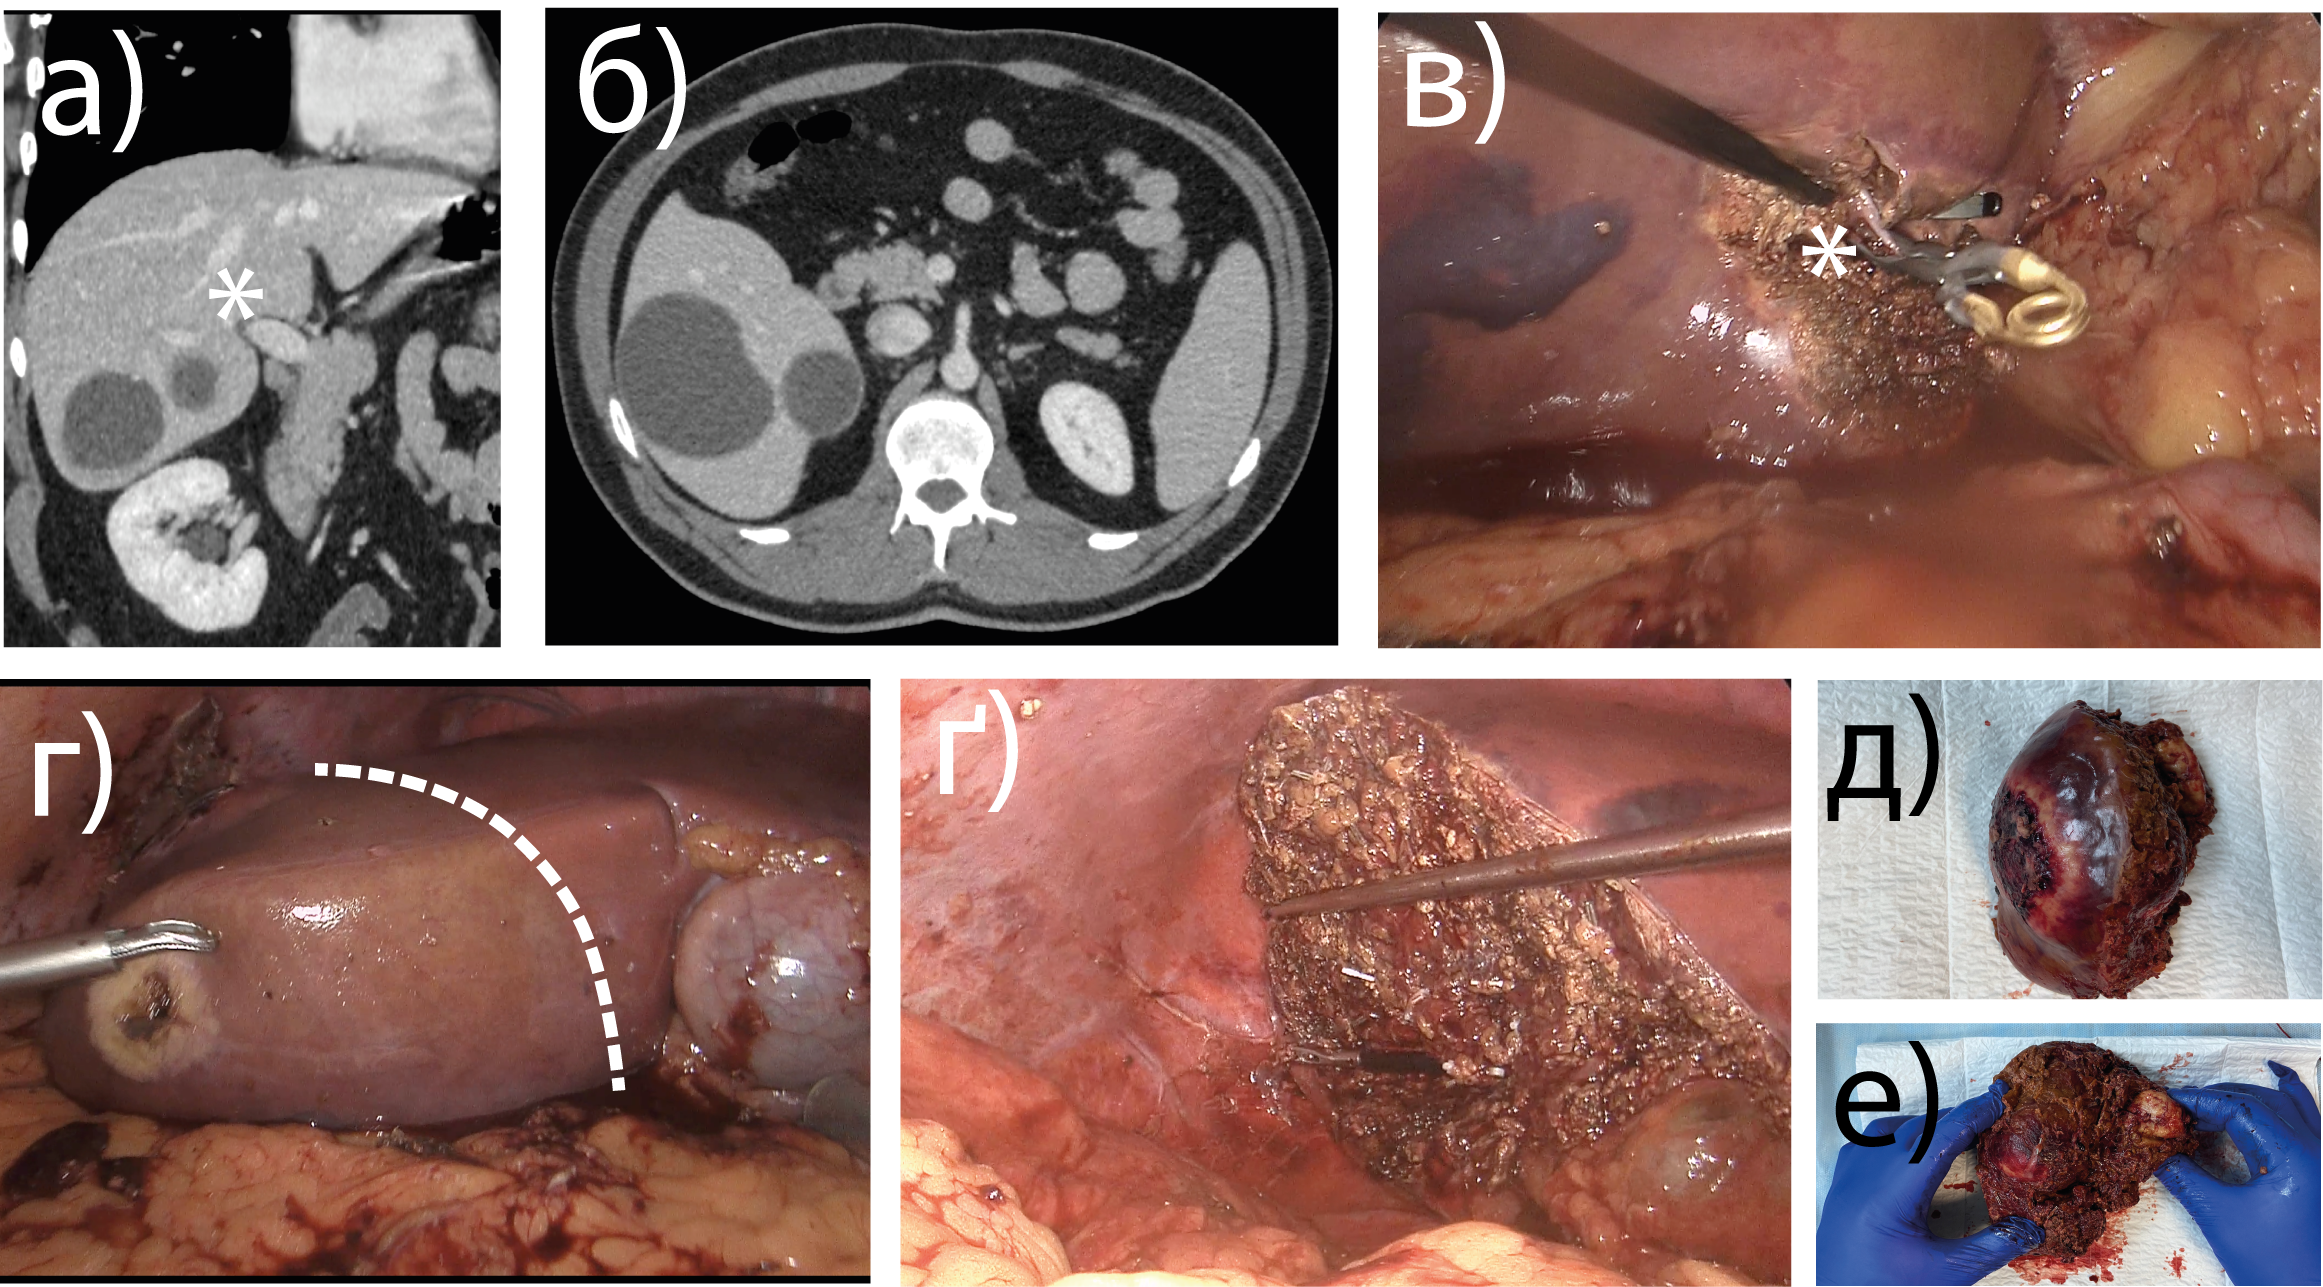
\includegraphics[width=0.95\textwidth]{Illustrations/Chapter_01/ECC-Sg6.png}
\label{fig:ECC-Sg6}

\medskip
\small
а,б) Передопераційне \acrshort{ct}. Ехінококові кисти розташовані в Sg 6 печінки та прилягають до сегментарного глісону (помічено зірочкою) в) Глісон Sg 6 виділено та кламповано г) Лінія демаркації після перетискання глісонової ніжки ґ) Площина резекції д,е) Макропрепарат  

\end{figure}



Анатомічна радикальна резекція печінки є методом вибору для лікування більш агресивної форми паразитарного ураження печінки - альвеолококозу. За данними нещодавнього метааналізу \acrshort{llr} є потенційно ефективними методом лікування цього захворювання при дотриманні показів, а його результати порівняні із виконанням відкритих втручаннь \cite{Salm2019}. 

\subsubsection{Первинний внутрішньопечінковий холелітіаз}

Первинний внутрішньопечінковий холелітіаз (\acrshort{pil}) є хронічним захворюванням, більш ендемічним для східноазіатських країн, проте може зустрічатись і в європейських країнах. Захворювання може проявляти себе больовим синдромом або періодичними симптомами холангіту. Для корректного визначення способу лікування потрібно диференційювати \acrshort{pil} із вторинним холелітіазом, який може бути наслідком міграції конкрементів з жовчного міхура або наслідком попередніх гепатобіліарних втручаннь. Механізм виникниння \acrshort{pil} чітко не з'ясований, але відомо, що у європейського населення він часто асоційований з 4 типом кіст біліарного дерева (хворобою Каролі), яка є показом до трансплантації печінки. Також відомо, що \acrshort{pil} частіше локалізується в лівій долі печінки, що пов'язують із більшим кутом лівого дольового протоку до холедоху та сповільнення пасажу жовчі в ньому \cite{Giuliante2015}.

Показано хороші результати застосування \acrshort{llr} для \acrshort{pil}, особливо при найбільш частій лівобічній локалізації. Так доступні результати південнокорейського порівняльного дослідження результатів лікування \acrshort{pil}. У дослідження були включені 149 пацієнтів із \acrshort{pil}, яким було виконано резекцію печінки відкритим та лапароскопічним шляхом, на основі аналізу результатів лікування яких автори дійшли висновку, що \acrshort{llr} є радикальним та безпечним методом лікування, який дозволяє знизити післяопераційну морбідність та асоційований із скороченням періоду реабілітації.